%%% lorem.tex --- 
%% 
%% Filename: lorem.tex
%% Description: 
%% Author: Ola Leifler
%% Maintainer: 
%% Created: Wed Nov 10 09:59:23 2010 (CET)
%% Version: $Id$
%% Version: 
%% Last-Updated: Wed Nov 10 09:59:47 2010 (CET)
%%           By: Ola Leifler
%%     Update #: 2
%% URL: 
%% Keywords: 
%% Compatibility: 
%% 
%%%%%%%%%%%%%%%%%%%%%%%%%%%%%%%%%%%%%%%%%%%%%%%%%%%%%%%%%%%%%%%%%%%%%%
%% 
%%% Commentary: 
%% 
%% 
%% 
%%%%%%%%%%%%%%%%%%%%%%%%%%%%%%%%%%%%%%%%%%%%%%%%%%%%%%%%%%%%%%%%%%%%%%
%% 
%%% Change log:
%% 
%% 
%% RCS $Log$
%%%%%%%%%%%%%%%%%%%%%%%%%%%%%%%%%%%%%%%%%%%%%%%%%%%%%%%%%%%%%%%%%%%%%%
%% 
%%% Code:

\chapter{Method}
\label{cha:method}

\section{Pre-processing}
\label{sec:pre-processing}
The data for this project was delivered by Östgötatrafiken. The whole dataset is over 300GB in size. The data contains, among other things, GPS coordinates and different types of events representing actions performed by a bus. To be able to feed the data into our models, preprocessing had to be done. The initial data exploration was performed by using jupyter notebooks and the python pandas package. Data operations such filtering and plotting the statistical distributions of the raw data provided an initial overview of the data set. By creating a simple finite state-machine, the data covering a complete journey from a specific bus line could be extracted.


\subsection{Data structure}
The provided data consists of 90 files, where each file represents one day of data. Each file has an approximate size of 5GB. Within the data there are over 20 event-types that represent the state of a bus during a day. For this project four types of events were used, while the others were discarded. The four events used are:
\begin{description}
\item[ObservedPositionEvent:] Gets triggered every second, contains the GPS data of a given bus.
\item[EnteredEvent:] Gets triggered when the bus is within a certain distance to a bus-station. Is used to split the journey into segments.
\item[JourneyStartedEvent:] Gets triggered when the bus is assigned a new journey. Is used to determine which line a bus is currently serving.
\item[JourneyCompletedEvent:] Gets triggered when the bus has completed a journey. Is used as a flag to determine when a journey has ended.
\end{description}

TODO (this section) For this project XXXX bus lines were selected: a subset of the bus line three and bus line number eleven. Line three has been used as a basis, since we all know that bus and we could assure that there were no irregularities on that line. Line eleven (Seen in Figure \ref{fig:211_stations}) had been chosen because it captures a lot of problems that need to be taken into consideration within our predictions. Such problems are GPS variance due to high buildings, high red light density, and down town traffic. 

\begin{figure}[t!]
\begin{minipage}{.5\textwidth}
	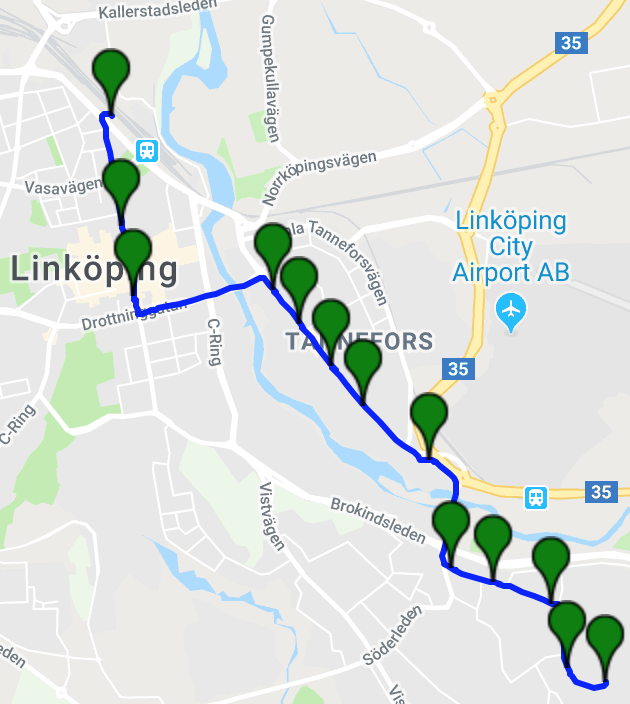
\includegraphics[scale=0.48,width=\textwidth]{211_stations}
	\caption{This figure shows a whole journey of the bus line 211. The markers in green are entered events. Those events have been used to segment the stations.}
	\label{fig:211_stations}
\end{minipage}
\hspace{5pt}
\begin{minipage}{.48\textwidth}
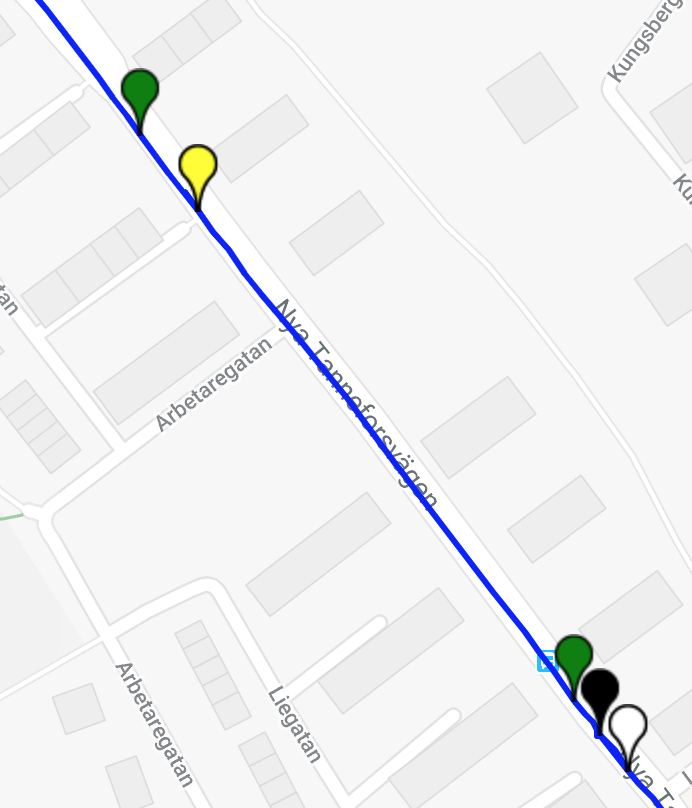
\includegraphics[scale=0.5,width=\textwidth]{entered}
\caption{This caption shows two stations,  the passed the upper left one without stopping, while in the lower right station the bus is stopping.}
\label{fig:entered}
\end{minipage}
\end{figure}


\subsection{Detecting Segments}
Bus journeys are split into several segments. The \textit{EnteredEvent} is used to detect when a bus is approaching a station, and is also used to split the raw data into segments.  We have first tried to use the \textit{StoppedEvent} for segment detection, but as seen in Figure \ref{fig:entered}, that event is not suitable for that use. Occasionaly, some stations are skipped because there are no people trying to get on or off the bus.
The first segment of a journey starts when a \textit{JourneyStartedEvent} triggers. When all the journeys of interest have been collected from the raw data, the collection is investigated in order to find and remove severe anomalies (such as drivers taking a wrong turn). These faulty journeys are discarded since it is not feasible to create a model which takes such complexity into consideration, given the amount of training data available.

\section{Baseline Method}
As a baseline method for segment time prediction the median for each segment over all training data has been used. TODO

\section{Artificial Neural Networks}
The neural network models were made using \textit{Keras} on top of \textit{Tensorflow}. A lot of models were created and different features were tested. There was a partly models as described by different papers and also some modified versions depending on what was available in the data.
All models will not be mentioned in this report, only the most significant ones. Featured models will be referenced by their notebook name.

\subsection{Special data pre-processing}
Common for all models is that test data is extracted as entire \textbf{journeys}, not as random samples. This allows for using a sequence of predictions with a Kalman filter.

\subsection{Model 1}\label{M1}
\textit{Notebook: Model 1 - sequence of test data}
\newline
\noindent This model was created based on the structure described by (blabla et al, Brazil pappret). The model predicts the time it takes to travel the current segment. It is assumed that the time is known when the bus left the latest station. Then, the time left to the next station is calculated by subtracting the time that has passed from the current station from the segment travel time prediction.

\subsubsection{Features}

\begin{itemize}
    \item Segment number (one-hot-encoded)
    \item Time of day (hour), normalized and (circled)<- bättre ord tack?
    \item Time traveld until current segment, normalized.    
\end{itemize}

\subsubsection{Layers}

\begin{itemize}
    \item 1 hidden fully connected layer - \textit{RelU activation}
    \item 1 output neuron
\end{itemize}


\subsection{Model 2}\label{M2}
\textit{Notebook: Model 2v2 - all data all features with sequence of test data}
\noindent This model directly predicts time left to the next station. This model lets the model do more abstraction work by providing more features. 

\subsubsection{Features}

\begin{itemize}
    \item Segment number (one-hot-encoded)
    \item Time of day (hour), normalized and (circled)<- bättre ord tack?
    \item Time traveld until current segment, normalized
    \item Bus direction (degrees), normalized and (circled)
    \item Bus speed (meter / second), normalized
    \item Bus position (latitude / longitude), normalized
\end{itemize}
  
%    \item Time of day (hour) normalized and (decircled)<- bättre ord tack?
%    \item Time traveld until current segment.
%    \item Direction of the bus
%    \item Speed of the bus
%    \item position of the bus

\subsubsection{Layers}

\begin{itemize}
    \item 1 hidden fully connected layer - \textit{RelU activation}
    \item 1 output neuron
\end{itemize}


\subsection{Model 3}
\textit{Notebook: Model 3v2 - all data all features w history}
\noindent This model is very similar to Model \ref{M2} with the addition of history from the three latest samples of position data. The idea is to let the model use this history to partly cope with dwell time.

\subsubsection{Features}

\begin{itemize}
    \item Segment number (one-hot-encoded)
    \item Time of day (hour), normalized and (circled)<- bättre ord tack?
    \item Time traveld until current segment, normalized
    \item Bus direction (degrees), normalized and (circled)
    \item Bus speed (meter / second), normalized
    \item Bus position (latitude / longitude), normalized
    \item Bus position history from 3 samples ago (latitude / longitude), normalized
\end{itemize}

\subsubsection{Layers}

\begin{itemize}
    \item 1 hidden fully connected layer - \textit{RelU activation}
    \item 1 output neuron
\end{itemize}

More is to be written..

%This model predicts the time it will take to travel to the next bus stop. As input this model use time of day normalized to a value in the range [0,1] and the segment for which the observation has been made. The segment input is one-hot encoded meaning that there is an input for each segment in the journey which all have a value of 0 except for the segment of the observation which has the value 1. The network has one fully connected hidden layer with 13 nodes and an output layer with one node. 
%The network uses the \textit{relu} activation function. This model predicts the time in seconds it will take to travel the whole segment. To get a prediction of the time to the next bus stop you need to subtract the actual known time travelled since the previous bus stop from the output of the neural network.

\subsection{Kalman filter}



%%%%%%%%%%%%%%%%%%%%%%%%%%%%%%%%%%%%%%%%%%%%%%%%%%%%%%%%%%%%%%%%%%%%%%
%%% lorem.tex ends here

%%% Local Variables: 
%%% mode: latex
%%% TeX-master: "demothesis"
%%% End: 
